%!TEX TS-program = xelatex
%!TEX encoding = UTF-8 Unicode

\documentclass{harvard-thesis}

\usepackage{float}
\usepackage{amssymb}
\usepackage{pifont}
\usepackage{url}

\usepackage[english]{babel}

\usepackage{geometry}
\usepackage{pdflscape}
\usepackage{booktabs}


\newcommand{\cmark}{\ding{51}}
\newcommand{\xmark}{\ding{55}}

\usepackage{adjustbox}
\usepackage{array}

\usepackage{amsfonts}

\usepackage{minted}
\usepackage{etoolbox}
\AtBeginEnvironment{minted}{\singlespacing%
    \fontsize{9}{9}\selectfont}
    
\newcolumntype{R}[2]{%
    >{\adjustbox{angle=#1,lap=\width-(#2)}\bgroup}%
    l%
    <{\egroup}%
}
\newcommand*\rot{\multicolumn{1}{R{45}{1em}}}

\usepackage{tikz}
\usetikzlibrary{arrows,shapes,positioning,shadows,trees}
\tikzset{
  basic/.style  = {draw, text width=5cm, drop shadow, font=\sffamily, rectangle},
  root/.style   = {basic, rounded corners=2pt, thin, align=center, fill=green!30},
  level 2/.style = {basic, rounded corners=6pt, thin,align=center, fill=green!60, text width=8em},
  level 3/.style = {basic, thin, align=left, fill=pink!60, text width=6.5em,font=\small}
}


\newtheorem{research-question}{Research question}
\newtheorem{research-sub-question}{Research sub-question}

\begin{document}

% New definition of square root:
% it renames \sqrt as \oldsqrt
\let\oldsqrt\sqrt
% it defines the new \sqrt in terms of the old one
\def\sqrt{\mathpalette\DHLhksqrt}
\def\DHLhksqrt#1#2{%
\setbox0=\hbox{$#1\oldsqrt{#2\,}$}\dimen0=\ht0
\advance\dimen0-0.2\ht0
\setbox2=\hbox{\vrule height\ht0 depth -\dimen0}%
{\box0\lower0.4pt\box2}}

% the front matter
% some details about the thesis
\title{Web-scale outlier detection}
\author{F. T. Driesprong}
\advisor{dr. A. Lazovik}

% about the degree
\degree{Master of Science}
\field{Computing Science}
\degreeyear{2015}
\degreemonth{September}

% about the university
\department{Faculty of Mathematics and Natural Sciences}
\university{University of Groningen}
\universitycity{Groningen}
\universitystate{Netherlands}
\maketitle
\copyrightpage
\abstractpage
\tableofcontents
%\authorlist
\listoffigures
\dedicationpage
\acknowledgments

\onehalfspacing

% incluude each chapter...
\begin{savequote}[78mm] 
Als ik zou willen dat je het begreep, had ik het wel beter uitgelegd. \qauthor{Johan Cruijff} 
\end{savequote}

\chapter{Introduction}

As said in the $17^{\text{th}}$ century: ``Whoever knows the ways of Nature will more easily notice her deviations; and, on the other hand, whoever knows her deviations will more accurately describe her ways'' \cite{bacon2010novum}. This statement illustrates that uncovering outliers is a concept that hasz interested people throughout history. The aim of this thesis is to explore modern web-scale techniques for detecting outliers in large and complex datasets produced in today's data-driven society.

First, Section \ref{sec1-motivation} will explain why this thesis subject is important and give an introduction to the topic of outlier detection and its use and value. Second, Section \ref{sec1-researchquestions} introduces the research questions and scope. The research is conducted at Quintor, which will be introduced in Section \ref{sec1-Quintor}. 

\section{Motivation \label{sec1-motivation}}
In today's world we have accumulated a truly staggering amount of data. Since the 1980s the total amount of data has doubled every 40 months \cite{Hilbert01042011}. This overwhelming growth of about 28\% per annum is clearly exponential \cite{6479953}. This increase of data is caused by a variety of factors, among which the increasing interconnectivity of machines through the use of (mobile) internet. Apart from these technical innovations, movements such as the Internet of Things (IoT) and social media have caused a continuous increase in the volume and detail of data \cite{holler2014from}. 

\begin{figure}[ht!]
\centering
\includegraphics[width=\textwidth]{figures/kbpspercapita.pdf}
\caption[Telecom capacity per capita]{Kilobytes per second optimally compressed telecom capacity per capita \cite{SIGN:SIGN584}. Telecom includes fixed and mobile, telephony and internet. \label{fig:growth}}
\end{figure}

Figure \ref{fig:growth} illustrates the growth of telecom capacity over the years per capita. A distinction has been made by The Organization for Economic Co-operation and Development (OECD), which is an international economic organization of 34 countries founded in 1961 in order to stimulate economic progress and world trade. OECD countries are in general well developed countries of which the GDP per capita is in the highest quartile. The figure shows that while in 2001 the average inhabitant of the developed OECD countries had an installed telecommunication capacity of 32kbps, in 2010 the access capacity of an individual inhabitant had already multiplied by a factor of 100 to 3200kbps \cite{SIGN:SIGN584}.

Besides the volume, data is shifting from static sets to a continuously changing nature \cite{1558609016}. The handling of such massive amounts of dynamic data is known as `big data', which comprises datasets whose sizes are far beyond the ability of commonly used software tools to capture, curate, manage, and process within a tolerable time frame \cite{bigdata}. Many definitions of big data exist, as we follow the definition \cite{Hashem201598}: `Big data is a set of techniques and technologies that require new forms of integration to uncover large hidden values from large datasets that are diverse, complex and of a massive scale'. To obtain insights from large amounts of data, different tooling is required. For example, most relational database management systems and desktop statistics are not up to the task, instead we need `massively parallel software running on tens, hundreds, or even thousands of servers' to process the data \cite{Jacobs:2009:PBD:1536616.1536632}.

The process of extracting valuable knowledge from the large and complex amounts data is known as data mining, defined as `the non-trivial extraction of implicit, formerly unidentified and potentially constructive information from data in databases' \cite{Zaiane99introductionto,Kantardzic:2002:DMC:581837}. The goal of data mining is to mine the so-called golden nuggets from the mountain of data \cite{1347303}. The golden-nuggets are observations which provide knowledge about the data. Outlier detection, a subdivision of Knowledge Discovery and Data mining (KDD) differs in the sense that it detects data which shows behavior that differs from the rest of the data, and which might possibly be a so-called golden nugget \cite{Chandola:2009:ADS:1541880.1541882}.

Outlier detection has been studied by the statistical community as early as the $19^{\text{th}}$ century to highlight noisy data from scientific data sets \cite{14786448708628471}. For example, for normally distributed data, the observations which lie outside three times the standard deviation are considered outliers \cite{9783540262565}. Another commonly used method is based on statistical models, where a wide range of tests are used to find the observations which do not fit the model \cite{barnett1994outliers}. Such parametric models are not always suitable for general purpose outlier detection as it is not always clear which distribution the data follows. Recent outlier detection algorithms observe the local neighbouring observations and determine the outlierness based on the differences of the local neighbourhood.

The term `anomaly' or `outlier' is an ambiguous term, therefore a definition is in place. First, an outlier, sometimes referred to as an anomaly, exception, novelty, fault or error is defined as;
\begin{itemize}
  \item ``An observation which deviates so much from other observations as to arouse suspicions that it was generated by a different mechanism.'' \cite{Enderlein1987}
  \item ``An outlying observation, or ‘outlier,’ is one that appears to deviate markedly from other members of the observation in which it occurs.'' \cite{Grubbs1969}
  \item ``An observation (or subset of observations) which appears to be inconsistent with the remainder of that set of data.'' \cite{barnett1994outliers}
  \item ``An outlier is a data point that deviates quantitatively from the majority of the data points, according to an outlier-selection algorithm.'' \cite{outlierselection}
\end{itemize}

We follow the last definition, as we believe it is of importance to prove quantitatively that the data point is different from the majority of the set. Outliers may be `surprising veridical data', as belonging to class $\mathcal{A}$, but actually situated inside class $\mathcal{B}$, so the true classification of the point is surprising to the observer \cite{John95robustdecision}. Outlier detection analysis in big data may lead to new discoveries in databases, but an outlier can also be noise---a faulty sensor, for example. Finding aberrant or disturbing observations in large collections is valuable and might be a subject for further investigation. Outlier detection has a variety of applications, among which:

\begin{description}
  \item[Log analysis] Applying outlier-detection on log files helps to uncover issues with the hard- or software of a server. Applying it to network or server logs can unveil possible hacking attempts. 
  \item[Financial transactions] In recent years, outlier detection within the financial world has drawn considerable attention in research \cite{Kanhere2014}. By the use of outlier detection on credit-card transactions it is possible to indicate credit card fraud or identity theft \cite{618940}.
  \item[Sensor monitoring] As sensors are becoming cheaper and more integrated in our world, outlier detection can be used to monitor the data and identify faulty sensors \cite{Fujimaki:2005:ASA:1081870.1081917}.
  \item[Noise removal] Outlier detection is often used for the preprocessing of data in order to clear impurities and discard mislabeled instances \cite{Brodley96identifyingand}. For example, before training a supervised model, the outliers are removed from the training-dataset, thus removing possible noisy observations or mislabeled data \cite{63857}.
  \item[Novelty detection] Novelty detection is related to outlier detection as a novelty is most likely different from the known data. An example application is the detection of new topics of discussion on social media \cite{Markou20032481,Markou20032499,SPC3:SPC3353}.
  \item[Quality control] ``Outlier detection is a critical task in many safety critical environments as the outlier indicates abnormal running conditions from which significant performance degradation may well result, such as an aircraft engine rotation defect or a flow problem in a pipeline. An outlier can denote an anomalous object in an image such as a land mine. An outlier may pinpoint an intruder inside a system with malicious intentions so rapid detection is essential. Outlier detection can detect a fault on a factory production line by constantly monitoring specific features of the products and comparing the real-time data with either the features of normal products or those for faults'' \cite{6416666}.
\end{description}

Introducing outlier detection into the realm of web-scale computing will introduce requirements on the architecture, data-storage and deployment of the application. The data center has become a major computing platform, powering not only internet services, but also a growing number of scientific and enterprise applications \cite{Zaharia:2011:DNO:2170444.2170461}. By deploying the outlier detection systems on a cloud architecture allows the system to scale its capacity according to the current needs. For example, when an outlier detection algorithm listens to a stream of financial transactions, it needs to scale up at Christmas due the increase of workload, and can be scaled down every Sunday freeing up resources which can be used by other services such as reporting.

It is difficult to determine if an observations is a true anomaly, but when marked as an outlier by the algorithm, it is probably worth further investigation the observation by a domain expert. Outlier detection is not new, but has not yet been widely implemented in a scalable architecture. From Quintors' perspective a shift in requirements becoming more evident each day. As the data changes faster, classical data warehousing/mining is not up to the job and a shift has to made to the realm of real-time processing \cite{1640284}. By providing real-time tactical support to drive actions that react to events as they occur. This requires shifting from batch-processing jobs to real-time processing. By real-time processing we refer to soft real-time whereby the added value of the results produced by a task decreases over time after the deadline expires \cite{259423}. The deadline is considered the expiration of the time span in which the result is expected.

\section{Research questions \label{sec1-researchquestions}}

The main focus of the thesis is on outlier detection within a scalable architecture, most standard outlier-detection algorithms do not consider an implementation on a web-scale level. Therefore the goal of this thesis is providing a scalable implementation which can be used in industry to apply outlier detection to very large data sets.

The research question and its sub-questions presented next will be supported, referred to and addressed throughout the thesis. By breaking the main question down into several sub-questions the different concerns can be isolated and addressed separately.

\begin{research-question} 
How to scale a general purpose outlier detection algorithms to a web-scale level. \label{req1}
\end{research-question}   

Outlier detection is part of the domain of Knowledge Discovery and Data mining (KDD). Most implementations are not developed with scalability in mind, but solely on the method to uncover outliers from the set of observations. Therefore the first question is to determine which algorithms can potentially benefit from a parallel implementation.

\begin{research-sub-question} 
Which general-purpose outlier detection algorithms can potentially be scaled out. \label{sub-req1}
\end{research-sub-question}

Scaling an algorithm out, or sometimes referred as scaling horizontally, is distributing the workload of the algorithm across different machines which will act as a single logical unit. The different methods of outlier detection needs examined to determine if it can be converted into a so called `embarrassingly parallel workload'. This requires the algorithm to be able to separate the problem into a number of parallel tasks which can be scheduled on a cluster of distributed machines.

\begin{research-sub-question} 
Which computational engines are appropriate for distributed outlier detection. \label{sub-req2}
\end{research-sub-question}

Recent years a variety of computational engines have been developed for developing distributed applications, mostly based on the MapReduce model \cite{Dean:2008:MSD:1327452.1327492}, such as Apache Hadoop\footnote{Apache Hadoop \url{http://wiki.apache.org/hadoop/HadoopMapReduce}}, Apache Spark \cite{Zaharia:2010:SCC:1863103.1863113}. Other frameworks, such as Apache Mahout\footnote{Apache Mahout \url{http://mahout.apache.org/}}, provide additional algorithms which run on top of computational engines. An overview will be given of available computational engines and their characteristics.


\begin{research-sub-question} 
How to adapt the algorithm to work with streams of data, rather than a static set. \label{sub-req3}
\end{research-sub-question}

Rather than mining outliers from a static set of data, data comes most of the time as a stream. Example streams are sensor data or transactions which arrive over time. Important to note is that data streams are likely to evolve over time.

\section{Quintor \label{sec1-Quintor}}
Quintor is a leading player in the fields of Agile software development, enterprise Java / .Net technology and mobile development. Since its foundation in the year 2005, Quintor has been growing steadily. From their locations in Groningen and Amersfoort, they provide support to their customers in facing the challenges that large-scale enterprise projects entail. Quintor has a software factory at its disposal, from where in-house projects are carried out. 

To our enterprise customers, Quintor provides services in the field of software development processes (Agile/Scrum), information analysis, software integration processes, automated testing, software development and enterprise architecture. Quintor provides full Agile development teams consisting of analysts, architects and developers.

From Quintors' perspective the area of big-data is experiencing a tremendous growth and companies are looking for ways to extract knowledge from their data to obtain strategic insights.

\begin{savequote}[75mm] 
Building things - because they needed to be built. \qauthor{Johan Basse Bergqvist} 
\end{savequote}

\chapter{Background \label{chap2:background}}
This chapter will provide insights of the background from the literature on both outlier detection in Section \ref{sec2:outlier} and web-scale techniques in Section \ref{sec2:webscale}.

\section{Outlier detection algorithms \label{sec2:outlier}}
Outlier detection algorithms aim to automatically identify those valuable or disturbing observations in large collections of data. First we identify the different classes of knowledge discovery algorithms \cite{Fayyad:1996:DMK:257938.257942}, which is also applicable to outlier detection algorithms:

\paragraph{Unsupervised} algorithms try to find a hidden structure or pattern within a set of unlabeled observations. Figure \ref{fig:unsupervised} illustrates this, the observations given to the algorithm are unlabeled so no assumptions can be made. At the example, clustering, which is a classical unsupervised task, is applied on the set of observations. The output of the algorithm is reduced to clusters and can be manually reviewed. One of the difficulties is that it is often hard to evaluate performance of such algorithms as there is no clear error-function. In the case of clustering, it is not clear how many clusters are hidden in the data. In the case of outlier detection, it will compare the observations based on similarity.

\begin{figure}[ht!]
\centering
\includegraphics[width=\textwidth]{figures/unsupervised.jpg}
\caption{Unsupervised learning}
\label{fig:unsupervised}
\end{figure}

\paragraph{Supervised} is the machine learning task of inferring a function from labeled training data \cite{9780262018258}. As depicted in Figure \ref{fig:supervised}, supervised methods require as input a set of observations accompanied with a label which indicates to which class the observation belongs. For example, a label which is either legitimate or fraudulent, to assign the observation to a specific class. The training-set is used by the algorithm to learn how to separate the different classes. Once the model is trained, it can be used to classify to an observation of which the label is unknown.
\begin{figure}[ht!]
\centering
\includegraphics[width=\textwidth]{figures/supervised.jpg}
\caption{Supervised learning}
\label{fig:supervised}
\end{figure}
A disadvantage of supervised learning with respect to outlier detection is that large amount of labeled data is needed to train the model. 

\paragraph{Semi-supervised} learning is between unsupervised and supervised learning. The algorithms consists of a supervised algorithm that makes use of unlabeled data for training, typically a small amount of labeled data with a large amount of unlabeled data.

The follow-up step in the process is to detect outliers based on the stream of observations. The outliers might tell something about the transaction to determine if it legit or possibly fraudulently. This information can be used when a transaction is made or a cash withdraw is done, it needs to be determined within a short amount of time if the transaction is trustworthy, otherwise the transaction might possibly be canceled.

The goal of outlier detection is to identify the observations or objects that, for some reason, do not fit well to the remainder of a data set. A commonly used rule of thumb is that observations deviating more than three times the standard deviation from the distribution are considered outliers \cite{9783540262565}. Obviously this is not a very sophisticated method as it takes a global decision which is not locally aware. Most of the time such a global outlier model leads to a binary decision of whether or not a given object is an outlier. Local methods typically compute unbound score of `outlierness'. These scores differ per algorithm in scale, range and meaning \cite{4053049}, but can be used to discriminate different levels of outliers or to sort them and take the top $k$-observations.


Within literature different classes of outlier detection algorithms exists:
\begin{description}
 \item[Statistical based] assumes that the given data set has a distribution model which can be approximated using a function \cite{Hadi2009}. Outliers are those points that satisfies a discordancy test in relation to the hypothesized distribution \cite{barnett1994outliers}. 
 \item[Distance based] unifies the statistical distribution approach \cite{Knorr:1997:UAM:782010.782021} by assuming that an observation is an inlier when the distance of the $k$ nearest points in the data set are smaller than $\delta$ \cite{Knorr98algorithmsfor}. An updated definition which does not require the distance $\delta$, but introduces $n$ which defines if point $p$ is an outlier if $n-1$ other points in the data set have a higher value for $D^{k}$ \cite{Ramaswamy:2000:EAM:335191.335437}. Where $D^{k}(p)$ is the sum of distance to the nearest $k$ observations with respect to $p$.
 \item[Density based] algorithms identifies an object as an outlier if the observation has a significantly lower density with respect to the density of the local neighbourhood \cite{Breunig:2000:LID:335191.335388,Breunig:2000:LID:342009.335388}.
\end{description}
Beside the above mentioned classes there are many domain specific outlier-detection algorithms, for example for tumor detection within MRI data \cite{991693} or an algorithm which detect interesting points within engineering data \cite{rog}.

Density based approaches are sometimes seen as a variant of the distance based approach, as they share characteristics \cite{Kriegel:2008:AOD:1401890.1401946}. As distance based algorithms consider an observation an outlier when there are fewer than $k$ other observations within $\delta$ distance  \cite{Knorr:1999:FIK:645925.671529,Knorr:2000:DOA:764212.764218}. Another definition is the top $n$-observations which have the highest average distance to $k$ nearest neighbours \cite{fastoutlier,Eskin02ageometric}. Density based algorithms take it one step further as it computes from the $k$-nearest observations their average distance to their $k$-nearest observations and compare it with their own distance to the $k$-nearest observations \cite{Schubert:2014:LOD:2560809.2560914}.

With respect to the available algorithm, a subsection has been made in Table \ref{tbl:overviewAlgorithms} with restrictions:
\begin{itemize}
  \item The algorithm must be general purpose and not applicable to a specific domain.
  \item Many classical statistical algorithms are limited to one or only a few dimensions \cite{overviewsurvey} and have been left out as they are not applicable anymore.
  \item The observations which is the input data of the algorithm consists of a $m$-dimensional feature vector ${\bf x}=[x_{1},\ldots,x_{m}] \in \mathbb{R}^{m}$.
\end{itemize}

\begin{table}[!ht]
\noindent\makebox[\textwidth]{%
\begin{tabular}{lll}
{\bf Algorithm} & {\bf Type} & {\bf Year} \\ \hline
HilOut \cite{fastoutlier} & Distance-based & 2002 \\
Local Outlier Factor (LOF) \cite{Breunig:2000:LID:335191.335388,Aggarwal:2003:FCE:1315451.1315460} & Density-based & 2000 \\
Fast-MCD \cite{Rousseeuw:1999:FAM:331435.331458} & Statistical-based & 1999 \\
Blocked Adaptive Computationally Efficient Outlier Nominators \cite{Billor2000279} & Statistical-based & 2000 \\
Local Distance-based Outlier Factor (LDOF) \cite{Zhang2009} & Distance-based & 2009 \\
INFLuenced Outlierness (INFLO) \cite{ranking} & Density-based & 2006 \\
No-name \cite{Ramaswamy:2000:EAM:335191.335437} & Distance-based & 2000 \\
No-name \cite{Bay:2003:MDO:956750.956758} & Distance-Based & 2011 \\
Connectivity-Based-Outlier-Factor (COF) \cite{Tang:2002:EEO:646420.693665} & Density-Based & 2002 \\
Local Outlier Probabilities (LoOP) \cite{Kriegel:2009:LLO:1645953.1646195} & Density-based & 2009\\
Local Correlation Integral (LOCI) \cite{citeulike:1156150} & Distance-based & 2003 \\
Angle-Based Outlier Detection (ABOD) \cite{Kriegel:2008:AOD:1401890.1401946} & Angle-based & 2008 \\
Stochastic Outlier Selection (SOS) \cite{MSU:CSE:00:2} & Distance-based & 2012 \\
Simplified Local Outlier Detection (Simplified-LOF) \cite{Schubert:2014:LOD:2560809.2560914} & Density-based & 2014 \\           
\end{tabular}
}
\caption{An overview of outlier-detection algorithms\label{tbl:overviewAlgorithms}}
\end{table}


All of the distance-based and density-based algorithms stated in Table \ref{tbl:overviewAlgorithms} work with euclidean distance which is most popular for continues features. For discrete features the euclidean distance could be replaced by the hamming distance. Also other asymmetrical features can be used if desired. 

A disadvantage over statistical based approaches are that it is parametric as it tries to model the data to a given distribution. Distance based methods have a computational complexity of $\mathcal{O}(n^{2})$ as the pair-wire distance between all objects are required which effectively yields an $n$ by $n$ distance matrix. This makes it difficult to apply the algorithm to very large data sets as the execution time grows to an unacceptable level. Another method to reduce the computational time is by the use of spatial indexing structures such as the KD-tree \cite{Bentley:1975:MBS:361002.361007}, R-tree \cite{Guttman:1984:RDI:971697.602266}, X-tree \cite{Berchtold:1996:XIS:645922.673502} etc. But these such data-structures are often hard to distribute across multiple machines.

Unfortunately the `curse of dimensionality' also applies to $\epsilon$-range queries and $k$-nearest neighbour search \cite{citeulike:12369622}. The effect of the dimensionality as manifests itself as the number of dimensions increases the distance to the nearest data point approaches the distance to the farthest data point \cite{Beyer99whenis}. When taking this to an extreme as in Equation \ref{eq:distlimit}, the distance between becomes less meaningless as the dimensionality increases as the difference between the nearest and the farthest point converge to zero \cite{meaningnearestneighbour,Hinneburg:2000:NNH:645926.671675,Aggarwal01onthe}.

\begin{equation}
\lim_{d \to \infty} \frac{\text{dist}_{\text{max}} - \text{dist}_{\text{min}}}{\text{dist}_{\text{min}}} \to 0
\label{eq:distlimit}
\end{equation}

Not only hinders the higher dimensionality ease of discriminating the distance between the different points, it also makes the outliers less intuitive to understand. For distance-based outlier algorithms there are ways to evaluate the validity of the identified outliers which helps to improve the understanding of the data \cite{Knorr:1999:FIK:645925.671529}. When the number of dimensions grows, this process becomes difficult and impossible in extremes.

The use of high-dimensional data depends on the context and cannot be generalized. High-dimensional data can improve accuracy when all the dimensions are relevant and the present noise is tolerable.

%Another option is to reduce the number of dimensionality which is converting data of high dimensionality into data of much lower dimensionality such that each of the lower dimensions convey much information. Typical techniques are Principal Component Analysis, Factor analysis, etc \cite{citeulike:5467879}.

\section{Web-scale computing \label{sec2:webscale}}

To allow the system to scale which is require to cope with increasing workload and gives the ability to process large amounts of data, web-scale technology is adopted. This typically involves the ability to seamlessly provision and add resources to the distributed computing environment. Web-scale is often associated with the infrastructure required to run large distributed applications such as Facebook, Google, Twitter, LinkedIn, etc. 

Scaling the computations to multiple machines will be done by adopting the cloud computing paradigm. Within literature different definitions of cloud computing have been proposed \cite{clouddef}, there is diversity as it does not comprise of a new technology, but rather a new model that brings together a set of existing technologies to develop and execute applications in a way that differs from the traditional approach \cite{zhang:cloud}. Currently web-scale architectures is an active field of research \cite{cherniack2003scalable}.

Web-scale applications rely on cloud computing which is one of the most significant shifts in modern IT for enterprise applications and has become a powerful architecture to perform large-scale and complex computing. Within literature, several definitions of cloud computing exists \cite{sathyavani}. The main reason behind the diversity of cloud computing is that it does not comprise of a new technology, but rather a new model that brings together a set of existing technologies to develop and execute applications in a way that differs from the traditional approach \cite{zhang:cloud}. Clouds are used for different purposes and have numerous application areas. We define a cloud as; `a large pool of easily accessible virtualized resources, which can be dynamically reconfigured to adjust to a variable load, allowing for optimum resource utilization' \cite{Vaquero:2008:BCT:1496091.1496100}. 

On top of the cloud-computing environment big-data techniques are used. The world of big-data consists of a wide range of tools and techniques, which address and solve different problems. A mapping of the different components is given in Figure \ref{fig:classification}. Our focus is on the data-processing part as our goal is to efficiently distribute the outlier detection algorithm onto a cluster of working nodes.

\begin{figure}[!ht]
\noindent\makebox[\textwidth]{%
    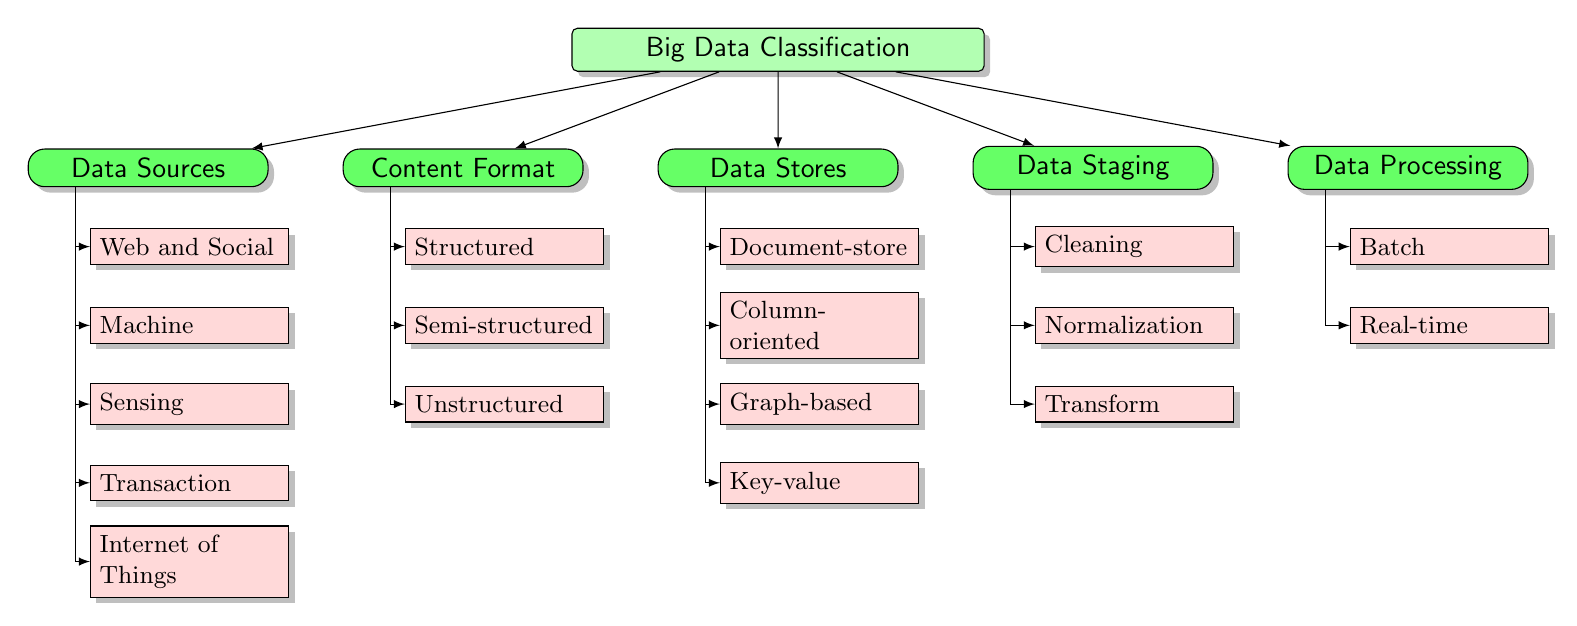
\begin{tikzpicture}[level 1/.style={sibling distance=40mm},edge from parent/.style={->,draw},>=latex]
    
    % root of the the initial tree, level 1
    \node[root] {Big Data Classification}
    % The first level, as children of the initial tree
      child {node[level 2] (c1) {Data Sources}}
      child {node[level 2] (c2) {Content Format}}
      child {node[level 2] (c3) {Data Stores}}
      child {node[level 2] (c4) {Data Staging}}
      child {node[level 2] (c5) {Data Processing}};
    
    \node [style=level 3, below of = c1, xshift=15pt] (c11) {Web and Social};
    \node [style=level 3, below of = c11] (c12) {Machine};
    \node [style=level 3, below of = c12] (c13) {Sensing};
    \node [style=level 3, below of = c13] (c14) {Transaction};
    \node [style=level 3, below of = c14] (c15) {Internet of Things};
    
    \node [style=level 3, below of = c2, xshift=15pt] (c21) {Structured};
    \node [style=level 3, below of = c21] (c22) {Semi-structured};
    \node [style=level 3, below of = c22] (c23) {Unstructured};
    
    \node [style=level 3, below of = c3, xshift=15pt] (c31) {Document-store};
    \node [style=level 3, below of = c31] (c32) {Column-oriented};
    \node [style=level 3, below of = c32] (c33) {Graph-based};
    \node [style=level 3, below of = c33] (c34) {Key-value};
    
    \node [style=level 3, below of = c4, xshift=15pt] (c41) {Cleaning};
    \node [style=level 3, below of = c41] (c42) {Normalization};
    \node [style=level 3, below of = c42] (c43) {Transform}; 
    
    \node [style=level 3, below of = c5, xshift=15pt] (c51) {Batch};
    \node [style=level 3, below of = c51] (c52) {Real-time};
    
    \foreach \value in {1,2,3,4,5}
      \draw[->] (c1.195) |- (c1\value.west);
    
    \foreach \value in {1,2,3}
      \draw[->] (c2.195) |- (c2\value.west);
    
    \foreach \value in {1,2,3,4}
      \draw[->] (c3.195) |- (c3\value.west);
      
    \foreach \value in {1,2,3}
      \draw[->] (c4.195) |- (c4\value.west);
      
    \foreach \value in {1,2}
      \draw[->] (c5.195) |- (c5\value.west);
    \end{tikzpicture}}
      
    \caption{Overview Big-Data landscape \cite{Hashem201598} \label{fig:classification}}
\end{figure}

Google introduced in 2008 the MapReduce computing model which provides a model for processing large data sets in a parallel and distributed fashion on a cluster of machines \cite{Dean:2008:MSD:1327452.1327492}. Google used it to scale their PageRank algorithm to serve personalized results to the users of their search engine \cite{Bahmani:2011:FPP:1989323.1989425}. The MapReduce model is a simple yet powerful model for parallelizing data processing. 

Microsoft launched in 2007 a data-processing system to write efficient parallel and distributed applications more easily under the codename Dryad \cite{export:63785}. DryadLINQ provides a set of language extensions that enable a new programming model for large scale distributed computing. A DryadLINQ program is a sequential program composed of LINQ expressions performing arbitrary side effect-free transformations on datasets \cite{export:70861}. In November 2011 Dryad had been discontinued active development and Microsoft shifted their focus to the Apache Hadoop project \cite{linqdisc}.

The Apache Hadoop project is an implementation of the MapReduce model. It is the open-source implementation primarily developed by Yahoo, where it runs jobs that produce hundreds of terabytes of data on at least 10,000 cores \cite{HadoopMapYahoo}. Since then it is adopted by a large variety of institutes and companies in educational or production uses, among others Facebook, Last.FM and IBM\footnote{Hadoop: PoweredBy \url{https://wiki.apache.org/hadoop/PoweredBy}}.

Although the name MapReduce originally referred to the proprietary Google technology, over the years it became the general term for the way of doing computations. The open-source implementation that has support for distributed shuffles is part of Apache Hadoop\footnote{Apache Hadoop \url{http://hadoop.apache.org/}}. A MapReduce job consists of three phases, namely Map, Combiner and Reduce \cite{Dean:2008:MSD:1327452.1327492}:

\begin{description}
  \item[Map] In the map phase operations on every individual record in the data set can be performed. This phase is commonly used to transform fields, apply filters or join and grouping operations. There is no requirement that for every input record there should be one output record.
  \item[Combine] For efficiency and optimization purposes it sometimes makes sense to suppla combiner class to perform a reduce-type function. If a combiner is used then the map key-value pairs are not immediately written to the output. Instead they will be collected in lists, one list per each key value. When a certain number of key-value pairs have been written, this buffer is flushed by passing all the values of each key to the combiner method and outputting the key-value pairs of the combine operation as if they were created by the original map operation.
  \item[Reduce] Before the reduce task it might be the case that distributed data needs to be copied to the local machine. When this is done, each with its corresponding values is passed to the reduce operation. 
\end{description}

First, input data is split into divided into parts and passed to the mapper which executes in parallel. The result is partitioned by key and locally sorted. Result of the data of the mapper of the same key will land on the same reducer and consolidated there. The merge sort happens at the reducer, so all keys arriving the same reducer is sorted.

There is a variety of open-source frameworks based or inspired on the MapReduce model, each with their own characteristics, which are commonly used for big-data processing:
\begin{description}
    \item[Apache Hadoop] is the open-source implementation of the propriety MapReduce model. The Apache Hadoop consists of four modules namely; First, the Hadoop MapReduce framework which consists of A YARN-based system for parallel processing of large data sets. Second, Hadoop Distributed File System (HDFS) in a distributed user-level file system which focuses on portability across heterogeneous hardware and software platforms \cite{5452045} inspired by the Google File System \cite{Ghemawat:2003:GFS:1165389.945450}. Third, Hadoop YARN which stands for Yet Another Resource Negotiator which is a framework for job scheduling and cluster resource management \cite{Vavilapalli:2013:AHY:2523616.2523633}. Last, Hadoop Common which provides the services for supporting the Hadoop modules.
    \item[Apache Spark] is the implementation of the concept of the Resilient Distributed Datasets (RDDs) developed at UC Berkeley \cite{180560}. RDDs are fault-tolerant, parallel data structures that persist intermediate results in memory and enables the developer explicitly control the partitioning to optimize data locality. Manipulate RDDs can be done using filters, actions and transformations by a rich set of operators. The concept of RDD is inspired by MapReduce and Dryad.
\end{description}

MapReduce is deficient in iterative jobs because the data is loaded from disk each iteration and interactive analysis because significant latency occurs because all the data has to be read from the distributed file system \cite{Zaharia:2010:SCC:1863103.1863113}. This is where Apache Spark steps in by storing intermediate results in-memory.

Hadoop provides fault-tolerance by the use of the underlying HDFS which replicates the data over different nodes. Spark does not store the transformed information between each step, but when a block of data gets lost, the original data is loaded and Spark reapplies all the transformations. Although it is possible to explicit save the state by enforcing a checkpoint.

By the use of this strategy Spark's in-memory primitives provide performance up to 100 times faster than Hadoop for certain applications \cite{Xin:2013:SSR:2463676.2465288}.
\begin{savequote}[90mm] 
Software is a great combination between artistry and engineering. \qauthor{Bill Gates} 
\end{savequote}

\chapter{Architecture \label{chap:architecture}}

This chapter describes the architecture on which the software is build and how its influence on the results. Figure \ref{fig:architecture} illustrates using course-grained blocks the architecture. The arrows illustrate the data-flow through the system. 

\begin{figure}[ht!]
\centering
\includegraphics[width=\textwidth]{figures/architecture.jpg}
\caption{Architecture of the system}
\label{fig:architecture}
\end{figure}

The emphasis of the architecture is on scalability. Meaning that it is simple to increase of decrease the number of worker nodes across a number of different physical machines as the machines are provisioned automatically. Tending to implement or evolved to an `elastic architecture' \cite{9780470887998}, which autonomously adapts its capacity to workload over time \cite{180145}, although the number of nodes is configured systematically to determine its performance for a set number of nodes. The underlying provisioning of the resources is done by Docker as described in section \ref{subsec_docker}. The input data on which the algorithm will perform the computations is kept in an Apache Kafka messaging system, described in section \ref{subsec_kafka}. Finally, the computational framework itself build upon Apache Spark is discussed in Section \ref{subsec_spark}.

\begin{figure}[ht!]
\centering
\includegraphics[width=.6\textwidth]{figures/asf.png}
\caption{Logo Apache Software Foundation}
\label{fig:asf}
\end{figure}

Most of the software on which the architecture is build is part of the Apache Software Foundation\footnote{Apache Software Foundation \url{http://www.apache.org/}}, which is a decentralized community of developers across the world. The software produced is distributed under the terms of the Apache License and is therefore free and open source software. The Apache projects are characterized by a collaborative, consensus-based development process and an open and pragmatic software license. 

\section{Docker \label{subsec_docker}}

Docker is an open-source project that automates the deployment of applications inside software containers\footnote{Docker \url{https://www.docker.com/}}. Docker uses resource isolation features of the Linux kernel to allow independent containers to run within a single Linux instance, avoiding the overhead of starting and maintaining virtual machines. Building on top of facilities provided by the Linux kernel, a Docker container, unlike a virtual machine, does not require or include a separate operating system. Docker also simplifies the creation and operation of task or workload queues and other distributed systems \cite{docker1,docker2}.

\begin{figure}[ht!]
\centering
\includegraphics[width=\textwidth]{figures/microservice.png}
\caption{Microservice architecture \cite{microservice} \label{fig:microservice}}
\end{figure}

Docker enables to encapsulate the different applications in lightweight-components which can easily be deployed on top of the docker daemon. This can be a single local docker-daemon or distributed across a pool of physical hosts. This enables deployment of the required components across a group of machines.

The Docker architecture is strongly inspired by the Microservice architecture as depicted in Figure \ref{fig:microservice}. Where every functionality is defined and encapsulated in its own container. Scaling such a system is done by adding or removing service. For example, if there is a computational intensive task scheduled on Spark, more docker-containers can be spawned on the pool of hosts to share the computational workload.

The stack is defined using Docker Compose\footnote{Docker Compose \url{https://www.docker.com/compose/}}, which is the successor of Fig\footnote{Fig \url{http://www.fig.sh/}}. Docker Compose is a tool for defining multi-container applications in a single file. The application with all the dependant containers will be booted using a single command which does everything that needs to be done to get it running.

At this moment Docker is used on a single machine, but can transparently scale to multiple host to create a clustering using Docker Swarm\footnote{Docker Swarm \url{https://docs.docker.com/swarm/}}. 


\section{Apache Spark \label{subsec_spark}}

Apache Spark\footnote{Apache Spark \url{http://spark.apache.org/}} is a computational platform which is designed to be distributed, fast and general purpose. It is an extension on the popular MapReduce model \cite{Dean:2008:MSD:1327452.1327492} and more efficient when it comes to iterative algorithms as it is able to performs in-memory computations \cite{Xin:2013:SSR:2463676.2465288}. Figure \ref{fig:sparkstack} illustrates the Apache Spark is running on top of Docker, but can also run standalone. Spark also includes libraries which specialize in special operation such as machine learning or graph-processing.

\begin{figure}[ht!]
\centering
\includegraphics[width=.9\textwidth]{figures/sparkstack.png}
\caption{Apache Spark stack \label{fig:sparkstack}}
\end{figure}

The computational model that Spark follows, consists generally of the following steps:

\begin{description}
  \item[Input-data] Spark is able to fetch the input-data from a variety of sources, including Hadoop Distributed File System, Amazon S3, Apache Flume, Apache Kafka, Apache HBase or any other Hadoop data source.
  \item[Transform] Transformations are defined based on the input data-set. Transformations can be for example, mapping the data to another format, joining different datasets or sorting the data into a specific order.
  \item[Aggregate] After the distributed transform of the data, everything is aggregated and loaded into the driver's local memory or is written to a persistent storage like HDFS.
\end{description}

Apache Spark works with Resilient Distributed Datasets (RDD), which is a read-only, partitioned collection of records. Each transformation within Spark uses a RDD as input and transforms the data into a new RDD. 

Apache Spark will only write to the file-system in a number of situations:
\begin{description}
    \item[Checkpoint] When setting a checkpoint on which it can recover from when data is lost because one or more machines in the clusters are unresponsive as result from a crash or network failure.
    \item[Memory] Every worker works with a subset of the RDD. When the subset grows in such a way that is does not fit in the memory anymore, the data will spill to disk.
    \item[Shuffle] When data needs to be shared across different worker-nodes a shuffle will occur. By designing and implementing an algorithm, these actions should be avoided or kept at an absolute minimum.
\end{description}

An important concept which needs to be taken into account is the number of partitions of a RDD. This is initially set by the source of the RDD. For example, for a \texttt{HadoopRDD} data-source which requests data blocks (64MB by default) from a Hadoop Distributed File System (HDFS), the number of spark-paritions set in park is equal to the number blocks \cite{Dean:2008:MSD:1327452.1327492}. This is a convenient way of managing the number of partitions as the number of partitions grows with the volume of the data. In the case of \texttt{KafkaRDD} which reads from Kafka`s distributed commit log, this is defined by the number of Kafka-partitions in the Kafka-cluster.

It is important to be aware of the number of partitions as it controls the parallelism of the submitted Spark Job. The number of partitions caps the number of tasks which can be executed in parallel. For example, if the RDD has only a single partition, there will be no parallel execution at all.

Spark recommends two or three partitions per CPU core in the cluster\footnote{Apache Spark: Level of Parallelism\url{http://spark.apache.org/docs/latest/tuning.html\#level-of-parallelism}}. This value is heuristically determined and in practice this values needs to be tunes to obtain optimal performance as it differs per type of task.

The Spark Streaming library\footnote{Spark Streaming \url{http://spark.apache.org/streaming/}} introduced in version 1.2 of Apache Spark makes it easy to build scalable fault-tolerant streaming applications. Spark Streaming uses micro-batch semantics, as illustrated in Figure \ref{fig:streaming}.

\begin{figure}[ht!]
\centering
\includegraphics[width=.9\textwidth]{figures/flow.png}
\caption{Spark streaming \label{fig:streaming}}
\end{figure}

By defining a window, for example, for example by a unit of time or per a fixed number of waiting messages. Each time the requirement is full-filled, a new job will be dispatched with as input the window. This streaming concept is particularly well suited using Apache Spark as the data-source.

\section{Apache Kafka \label{subsec_kafka}}

Apache Kafka\footnote{Apache Kafka \url{http://kafka.apache.org/}} provides functionality of a messaging queue in a distributed, partitioned and replicated messaging fashion. Figure \ref{fig:kafka} illustrates the role of Kafka. First, the terminology will be established, which is analogously to message queue's in general:

\begin{description}
    \item[Broker] is a process running on a machine which form together the Kafka cluster. 
    \item[Producer] is a process which publishes messages to the Kafka cluster.
    \item[Consumer] is a process that is subscribed to topics and reads the feed of published messages.
    \item[Topics] is a category identified by a string on which the messages are collected. Each producer and consumer can subscribe to one or more topics on which is writes or reads messages.
    \item[Partition] Each topic is divided into a set of partitions to distribute the topic across a set of different machines.
\end{description}

Producers are in the role of pushing messages into the log and the consumers read the log as messages are appended to the topics which are distributed across multiple machines to split the workload and volume of the data across a number of machines. The high-level topology of an Apache Kafka is given in Figure \ref{fig:kafka}, where three producers which publish messages to the cluster and the three consumers which receive the messages on the topics they are subscribed to.

\begin{figure}[ht!]
\centering
\includegraphics[width=.7\textwidth]{figures/kafka.png}
\caption{Apache Kafka high-level topology. \label{fig:kafka}}
\end{figure}

Apache Kafka is implemented as a distributed commit log, an immutable sequence of messages that is appended as new messages arrive, as illustrated in Figure \ref{fig:kafkalog}. Each messages in the partitions are each assigned a sequential id number called the offset that uniquely identifies each message within the partition. They allow the log to scale beyond a size that will fit on a single server. By default the partitioning is done in a round-robin fashion, but a partitioning algorithm can be implemented to enhance data-locality. 

\begin{figure}[ht!]
\centering
\includegraphics[width=.9\textwidth]{figures/kafkalog.jpg}
\caption{Anatomy of a topic, implemented as a distributed commit log\label{fig:kafkalog}.}
\end{figure}

The performance is effectively constant with respect to data size, so retaining lots of data is not a problem respecting the limitation of fitting a single partition on a single broker. Each partition can be replicated across a configurable number of brokers to ensure fault tolerance and availability of the Kafka cluster.

Apache Kafka allows producers to write arrays of bytes as a record. This means that serializing and deserializing the Scala data-structures has to be done by the programmer. This is done is done in an easy and fast way using the Pickling\footnote{Scala Pickling \url{https://github.com/scala/pickling}} library. 

\section{Apache ZooKeeper \label{subsec_ZooKeeper}}

ZooKeeper\footnote{Apache ZooKeeper \url{https://zookeeper.apache.org/}} is a highly-available coordination service for maintaining configuration, naming, distributed synchronization and providing group services \cite{Hunt:2010}. All of these kinds of services are used in some form or another by distributed applications, including Apache Kafka and Apache Spark. Because of the difficulty of implementing these kinds of distributed services, applications initially usually skimp on them, which make them brittle in the presence of change and difficult to manage. Even when done correctly, different implementations of these services lead to management complexity when the applications are deployed. This is where ZooKeeper steps in.

\begin{figure}[ht!]
\centering
\includegraphics[width=.9\textwidth]{figures/zookeeper.png}
\caption{ZooKeeper topology. \label{fig:ZooKeeper}}
\end{figure}

As depicted in Figure \ref{fig:ZooKeeper}, the ZooKeeper service comprises an ensemble of servers that use replication to achieve high availability and performance. ZooKeeper provides a shared hierarchical name-space which is consistent across all nodes. ZooKeeper runs in memory which ensures high throughput and low-latency.

ZooKeeper replicates the name-space across all nodes using a transaction-log which ensures that all the mutations performed by the majority of the ZooKeeper-instances in the cluster. The operations on ZooKeeper are wait-free and does not uses blocking operations such as locks. This is implemented in the leader-based atomic broadcast
protocol named ZooKeeper Atomic Broadcast (ZAB) \cite{zab} which implements the following guarantees \cite{Hunt:2010}:

\begin{description} 
    \item[Linearizable writes] all requests that update the state of ZooKeeper are serializable and respect precedence.
    \item[FIFO client order] all requests from a given client are executed in the order that they were sent by the client.
\end{description}

As long as a majority of the servers are correct, the ZooKeeper service will be available, with a total of $2f+1$ Zookeeper processes, it is able to tolerate $f$ failures. When the cluster becomes partitioned, from for example a network failure, the partitions with the number of processes smaller than $f$ will become available and falls down to an auto-fencing mode, rendering the service unavailable \cite{0201619180}.

An interesting and useful feature of ZooKeeper are ephemeral nodes. These are nodes in the hierarchical name-space of the ZooKeeper service which will be removed as the process which created them disconnects of becomes unavailable. This enables the ZooKeeper service to only show the list of nodes which are available.

In the software-stack used for the experiment, ZooKeeper is used for:
\begin{description} 
    \item[Apache Kafka] a master is elected for each partition within a topic. This is needed if a partition is replicated, one master is assigned which the slaves will follow, if the master dies a new master gets elected out of the slaves. 
    \item[Apache Spark] Spark allows to have multiple masters of which only one is active. If the master dies, a standby-master can take over and resubmit the job.
\end{description}

\section{Software}

The software will be written on top of the architecture as described above. The software will use the Spark Driver to communicate with the cluster. The way this works is illustrated in Figure \ref{fig:driver}. Instead of submitting a packed program to the cluster, the driver tells the worker nodes where the data is and the transformations are serialized and transferred to the worker nodes.

\begin{figure}[ht!]
\centering
\includegraphics[width=\textwidth]{figures/clusterdriver.png}
\caption{Spark context which sends the job to the worker nodes. \label{fig:driver}}
\end{figure}

The Spark-driver will also be deployed on the server as a Docker container. This will ensure that the driver will run on the same cluster and network communication between cluster and the executors will be minimal.

The software is build using Simple Build Tool\footnote{Simple Build Tool \url{http://www.scala-sbt.org/}} (SBT) which handles the flow of testing, running and packaging. Using the SBT Assembly plugin \footnote{SBT Assembly \url{https://github.com/sbt/sbt-assembly}} a JAR file is generated which contains all the source and the libraries it depends on. By packing specific versions of the dependant libraries into the JAR prevents the need of additional libraries to be available at run-time.

The source of the algorithm is placed in a GIT\footnote{GIT Version Control \url{https://git-scm.com/}} version control system called Github\footnote{Github \url{https://github.com/rug-ds-lab/SparkOutlierDetection}}, which keeps track of changes to the source code. The Github allows the developer to attach hoops to events, such as the push of new code to the repository.

As continuous integration server Travis\footnote{Travis CI \url{https://travis-ci.org/rug-ds-lab/SparkOutlierDetection}} is used to build a new version of the software each time a new push is done to the Github repository. The test-coverage of the software is tracked using Codecov\footnote{Codecov \url{https://codecov.io/github/rug-ds-lab/SparkOutlierDetection}}. Using Codecov the test-coverage is visualized per line of code, and gives suggestions which files require additional test-coverage. 
Codacy\footnote{Codacy \url{https://www.codacy.com/app/fokko/SparkOutlierDetection}} is used to keep track of the quality of code by performing static analysis on the code, each time changes are applied the code is searched for Scala specific code-smells which might incur errors, such as the creation of threads instead of using futures, the use of reserved key-words, high cyclomatic complexity or the use of \texttt{var} instead of the immutable \texttt{val}. 

\begin{savequote}[75mm] 
Talk is cheap. Show me the code. \qauthor{Linus Torvalds} 
\end{savequote}

\chapter{Algorithm \label{chap4:algorithm}}

This chapter introduces and differentiates between two types of algorithms that have been evaluated from the literature in Section \ref{sec2:outlier}. The algorithms presented in Table \ref{tbl:overviewAlgorithms} are distance based algorithms. For simplicity we use Euclidean distance, as in Equation \ref{eq:euclidean}, but all algorithms also work with other metrics. For example, metrics such as the Hamming distance, which can find the number of different symbols in strings of equal length and which is often used for comparing bit-sequences \cite{citeulike:1667687}. Another distance-function is the Levenshtein distance, which is used for comparing different strings of text. The Euclidean distance between observation $a$ and $b$ is the length of the line segment connecting them, and is therefore intuitive for people to grasp \cite{Deza2009EncyclopediaofDistances}.

\begin{equation}
d({\bf a},{\bf b}) = \sqrt{\sum^{m}_{i=1} (a_{i} - b_{i})^2} \label{eq:euclidean}
\end{equation}

The distance-based algorithm is related to the concept of clustering. An outlier can be seen as an observation which is not part of a cluster. Also, the algorithms take the locality into account. For example, for the Local Outlier Factor (LOF) algorithm, which compares the density of the surrounding neighbours, it is important to note that the global density may vary a lot across the feature space. Section \ref{sec:lof} introduces the Local Outlier Factor algorithm, which introduces the concept of local densities and which has been extended and adapted by many papers. This algorithm gives a good idea what outlier detection is about. Next, the Stochastic Outlier Selection (SOS) algorithm is introduced in Section \ref{sec:sos} and it elaborates on why it is a good fit for Apache Spark and LOF is not.

For outlier detection algorithms, there is no free lunch \cite{Wolpert95nofree}, which implies that there is no algorithm which outperforms all other algorithms \cite{outlierselection}. Different algorithms excel under different conditions, depending on the characteristics of the data set.

\section{Local Outlier Factor \label{sec:lof}}

Many distance-based outlier detection algorithms are based or strongly inspired by the Local Outlier Factor algorithm. The concept is depicted in Figure \ref{fig:lof}, where the black dots are the observations in the feature space and the dashed circles are the corresponding distances to the $k^{\text{th}}$-observation which is set to $k=3$.

\begin{figure}[ht!]
\centering
\includegraphics[width=.6\textwidth]{figures/lof.png}
\caption{Local Outlier Factor with $k=3$. \label{fig:lof}}
\end{figure}

First, the distance to the $k^{\text{th}}$-nearest observations is computed. This is called the Local Reachability Distance (LDR), as defined in Equation \ref{eq:reachability}, where $k\text{-distance}(A)$ is the distance to the $k^{\text{th}}$-nearest observation of the neighbouring observation $A$. 

\begin{equation}
\text{LDR}_{k}(A) = 1 / \left( \frac{\sum_{B \in N_{k}(A)} max(k\text{-distance}(B), d(A,B))}{|N_{k}(A)|} \right) \label{eq:reachability}
\end{equation}

After computing LDR for each observation, which requires the $k$-nearest neighbours and the $k$-nearest neighbors of the $k$-nearest neighbors, the Local Outlier Factor value can be obtained using Equation \ref{eq:lof}, which essentially compares the density of the observation itself with the density of the surrounding observations.

\begin{equation}
\text{LOF}_{k}(A) = \left( \frac{\sum_{B \in N_{k}(A)} \text{LDR}(B)}{|N_{k}(A)|} \right) / \text{LDR}(A)
\label{eq:lof}
\end{equation}

The algorithm relies heavily on nearest-neighbour searches which are hard to optimize on distributed computational platforms as they require searching through and sort all the data. Therefore the algorithm is not suitable to implement on top of Apache Spark.

\section{Stochastic Outlier Selection \label{sec:sos}}

Instead of comparing local densities, as done by the Local Outlier Factor concept, the Stochastic Outlier Selection algorithm employs the concept of affinity which does comes from the field of \cite{ictdbid:2777,AISTATS09_Maaten}:
\begin{description}
  \item[Clustering] employs affinity to quantify the relationships among observations \cite{Frey2007}. For example, the concept of affinity been used for partitioning protein interactions \cite{pmid19331680} and clustering text \cite{10.1109/TKDE.2010.144}.
  \item[Dimensionality reduction] Stochastic Neighbor Embedding \cite{NIPS20022276} or t-distributed Stochastic Neighbor Embedding \cite{van2008visualizing,ictdbid:2777} is a nonlinear dimensionality reduction technique for embedding high-dimensional data into a space of two or three dimensions. The technique has been used among music analysis \cite{Hamel+al:2010} and bio-informatics \cite{journals/bioinformatics/WallachL09}.
\end{description}

The implementation of the Stochastic Outlier Selection algorithm has been done in Scala\footnote{Scala programming language \url{http://www.scala-lang.org/}} on top of Apache Spark. To determine the correct working of the algorithm, unit-tests have been written in order to ensure correct output in each stage in the algorithm. The output of the implementation is compared to the output generated by the Python implementation written by the author\footnote{SOS \url{https://github.com/jeroenjanssens/sos/blob/master/bin/sos/}}. These unit-tests uncovered a bug in the authors' script, which has been patched by submitting a pull request\footnote{Github pull request \url{https://github.com/jeroenjanssens/sos/pull/4/}}.

The algorithm consists of a series of transformations on the data as described in the original paper \cite{MSU:CSE:00:2}. These steps are elaborated in the following subsections, which describe how they are implemented.

\subsection{Distance matrix \label{subsec:distancematrix}}
The distance matrix takes the $n$ input vectors of $m$ length and transforms it to a $n \times n$ matrix by taking the pairwise distance between each vector. We employ the symmetric Euclidean distance, as defined earlier in Equation \ref{eq:euclidean}. Being symmetric, the sets' distance $d({\bf x}_{i},{\bf x}_{j})$ is equal to $d({\bf x}_{j},{\bf x}_{i})$ and the distance to self is zero $d({\bf x}_{i},{\bf x}_{i}) = 0$. The distance matrix is denoted by ${\bf D}$, each row by ${\bf D}_{i} \in \mathbb{R}^{m}$ and each element by $D_{ij} \in \mathbb{R}$.

\begin{listing}[ht!]
\begin{minted}[frame=lines]{scala}
def computeDistanceMatrixPair(data: RDD[(Long, Array[Double])]): 
                                        RDD[(Long, Array[Double])] =
    data.cartesian(data).flatMap {
      case (a: (Long, Array[Double]), b: (Long, Array[Double])) =>
        if (a._1 != b._1)
          Some(a._1, euclDistance(a._2, b._2))
        else
          None
    }.combineByKey(
        (v1) => List(v1),
        (c1: List[Double], v1: Double) => c1 :+ v1,
        (c1: List[Double], c2: List[Double]) => c1 ++ c2
      ).map {
      case (a, b) => (a, b.toArray)
    }
\end{minted}

\caption{Computing the distance matrix of a collection of feature vectors.}
\label{list:matrixDistance}
\end{listing}

The implementation given in Listing \ref{list:matrixDistance} takes the Cartesian product of the input vectors to compute the distance between ever pair of observations. Next, the pairs are mapped to compute the Euclidean distance between every pair of vectors except to itself, as this does not carry any information and is not used by the algorithm. Finally, all the vectors are combined by the unique key of each vector returning the rows of the matrix.

\subsection{Affinity matrix \label{subsec:affinity}}
The affinity matrix is obtained by transforming the distance matrix proportionally to the distance between two observations. The affinity quantifies the relationship from one observation to another. The affinity $\sigma_{i}$ for each observation is found by performing a binary search, which makes the entropy of the distribution between overall neighbors equal to the logarithm of the perplexity parameter $h$.

\begin{equation}
a_{ij} = \begin{cases} \exp(-d_{ij}^{2} / 2 \sigma_{i}^{2}) & \text{if } i \neq j\\ 0 & \text{if } i = j \end{cases}
\label{eq:affinity}
\end{equation}

The perplexity parameter is the only configurable parameter of the algorithm denoted by $h$ as in Equation \ref{eq:perplexity}. The influence of the $h$ parameter is comparable to the $k$ parameter in the $k$-nearest neighbours algorithm. It also alters the behaviour of the algorithm analogously: the higher the value $h$, the more it depends on the surrounding neighbours. One important difference is that $h \in \mathbb{R}$ and $k \in \mathbb{N}$. The perplexity value has a deep foundation in information theory, but in practice should it be tuned by the domain expert to provide a good level of outlierness \cite{MSU:CSE:00:2}.

\begin{listing}[ht!]
\begin{minted}[frame=lines]{scala}
def computeAffinityMatrix(dMatrix: RDD[(Long, Array[Double])], 
                          perplexity: Double = DEFAULT_PERPLEXITY): 
                                  RDD[(Long, DenseVector[Double])] = 
  dMatrix.map(r => (r._1, binarySearch(new DenseVector(r._2), Math.log(perplexity))))
\end{minted}
               
\caption{Transforming the distance matrix to the affinity matrix.}
\label{list:matrixAffinity}
\end{listing}

Listing \ref{list:matrixAffinity} applies the binary search on each row within the matrix which approximates the affinity. The maximum number of iterations in the binary search can be limited in order to interrupt the execution which will introduce some error, but will reduce the computational time. Similar, an accepted tolerance can be set to accept a small error in exchange for reduced computational time. The binary search iteratively bisects the interval and then selects the correct upper of lower half until the desired variances for each observation is found.

\begin{equation}
h = \{x \in \mathbb{R} | 1 \leq x \leq n-1\}
\label{eq:perplexity}
\end{equation}

The affinity matrix is obtained by applying Equation \ref{eq:affinity} on every element of the distance matrix. Perplexity is employed to adaptively set the variances which are computed using the introduced binary search, which approximates for every value the $\sigma^{2}$ so that every observation has effectively $h$ neighbours \cite{NIPS20022276}. This has to be done for every observation assuming that it has a unique place in space. 

\begin{listing}[ht!]
\begin{minted}[frame=lines]{scala}
def binarySearch(affinity: DenseVector[Double],
                 logPerplexity: Double,
                 iteration: Int = 0,
                 beta: Double = 1.0,
                 betaMin: Double = Double.NegativeInfinity,
                 betaMax: Double = Double.PositiveInfinity,
                 maxIterations: Int = DEFAULT_ITERATIONS,
                 tolerance: Double = DEFAULT_TOLERANCE): DenseVector[Double] = {

  val newAffinity = affinity.map(d => Math.exp(-d * beta))
  val sumA = sum(newAffinity)
  val hCurr = Math.log(sumA) + beta * sum(affinity :* newAffinity) / sumA
  val hDiff = hCurr - logPerplexity

  if (iteration < maxIterations && Math.abs(hDiff) > tolerance) {
    val search = if (hDiff > 0)
      (if (betaMax == Double.PositiveInfinity || betaMax == Double.NegativeInfinity)
        beta * 2.0
      else
        (beta + betaMax) / 2.0, beta, betaMax)
    else
      (if (betaMin == Double.PositiveInfinity || betaMin == Double.NegativeInfinity)
        beta / 2.0
      else
        (beta + betaMin) / 2.0, betaMin, beta)

    binarySearch(   affinity,
                    logPerplexity, 
                    iteration + 1, 
                    search._1, 
                    search._2, 
                    search._3, 
                    maxIterations, 
                    tolerance)
  }
  else
    newAffinity
}
\end{minted}
\caption{Performing a binary search to approximate the affinity for each observation.}
\label{list:approximateAffinity}
\end{listing}

Listing \ref{list:approximateAffinity} shows the recursive function used to find or approximate the perplexity of each row $x_{i}$ in the distance matrix. The recursive function eliminates mutable variables which are impossible to avoid when using using loops. The use of immutable variables comes from the functional programming aspect of Scala and makes the code less error-prone.

\subsection{Binding probability matrix \label{subsec:bindingprob}}

The binding probability matrix defines the probability of observation $x_{i}$ to $x_{j}$. The mathematical foundation, based on graph theory, computes the Stochastic Neighbour Graph and the subsequent generative process is out of scope and can be found in the original paper \cite{MSU:CSE:00:2}.

\begin{equation}
b_{ij} = \frac{a_{ij}}{\sum_{k=1}^{n}a_{ik}}
\label{eq:binding}
\end{equation}

The binding probability matrix can be applied by normalizing the affinity matrix such that $\sum_{k=1}^{n}$ sums up to $1$. Equation \ref{eq:binding} transforms the affinity matrix to the probability outlier matrix.

\begin{listing}[ht!]
\begin{minted}[frame=lines]{scala}
def computeBindingProbabilities(rows: RDD[(Long, DenseVector[Double])]): 
                                            RDD[(Long, Array[Double])] = 
  rows.map(r => (r._1, r._2 :/ sum(r._2)).toArray)
\end{minted}

\caption{Transforming the affinity matrix into the binding probability matrix.}
\label{list:matrixProbability}
\end{listing}

Listing \ref{list:matrixProbability} shows the implementation which divides each element by the sum of the vector.

\subsection{Computing outlier probabilities \label{subsec:outlierprobabilities}}

The last step is to compute the outlier probability of vector ${\bf x}_{i}$, which is given by the product of the column binding probability matrix as in Equation \ref{eq:final}.

\begin{equation}
f{_\text{SOS}}({\bf x}_{i}) \equiv \prod^{n}_{\substack{i=1\\j \neq i}}(1-b_{ji}) \label{eq:final}
\end{equation}

The implementation is given in Listing \ref{list:matrixOutput}. The implementation uses a \texttt{flatmap} to add indices to the elements of the vector. The inline if-condition offsets the indices by one to skip the diagonal of the matrix. Important to note is the \texttt{zipWithIndex} operation is applied to the local collection and not on the RDD which would trigger a subsequent Spark job.

\begin{listing}[ht!]
\begin{minted}[frame=lines]{scala}
def computeOutlierProbability(rows: RDD[(Long, Array[Double])]):
                                                    RDD[(Long, Double)] =
  rows.flatMap(r => r._2.zipWithIndex.map(p =>
    (p._2 + (if (p._2 >= r._1) 1L else 0L), p._1))).foldByKey(1.0)((a, b) => a * (1.0 - b))
\end{minted}

\caption{Computing the outlierness from the binding probability matrix.}
\label{list:matrixOutput}
\end{listing}

Finally the \texttt{foldByKey} groups all the keys and perform a fold which computes the product of each column. This last action invokes a data-shuffle, as the rows are distributed across the different worker nodes. The product represents the outlierness of each observation.
\begin{savequote}[75mm] 
Nulla facilisi. In vel sem. Morbi id urna in diam dignissim feugiat. Proin molestie tortor eu velit. Aliquam erat volutpat. Nullam ultrices, diam tempus vulputate egestas, eros pede varius leo.
\qauthor{Quoteauthor Lastname} 
\end{savequote}

\chapter{Results \label{chap5:results}}

This chapter will present the quantitative results of the algorithm given in Chapter \ref{chap4:algorithm} on the software stack as presented in Chapter \ref{chap3:architecture}. First, Section \ref{sec:dataset} shows the data used for producing the results. Second, in Section \ref{sec:hardware} the hardware is presented on which the software stack runs. Finally, in Section \ref{sec:results} the tests and the results will be presented.

The purpose of this section is to perform empirical to explore the scalability of the algorithm based on input sets.

\section{Data-set \label{sec:dataset}}

The data-set is a synthetic which is generated at forehand. The input of the algorithm is a $m$ dimensional vector as in Equation \ref{featureVector}.

\begin{equation}
\textbf{x} = [x_{1},\ldots,x_{m}] \in \mathbb{R}^{m} \label{featureVector}
\end{equation}

The value of each feature vector is sampled in a pseudo-random fashion from a Gaussian distributed (also known as the normal distribution), shown in Figure \ref{gaussianDistribution}. The main characteristic of this distribution is when taken a theoretical infinite number of samples, approximately $68.2\%$ of the sampled values are within the $\pm 1$ standard deviation.

\begin{figure}[ht!]
\centering
\includegraphics[width=\textwidth]{figures/bellcurve.png}
\caption[Standard normal distribution]{The curve from which the feature vectors are sampled, the vertical-axis is the probability. The $\sigma$ values depict the standard deviations. \label{gaussianDistribution}}
\end{figure}

This will result in a data-set where the number of outliers will be limited as the mean of all the observation in the feature space will be at the origin. This will be not a problem as the goal is to determine the scalability of the algorithm and not its performance on determine if the observation is an outlier or not.

\section{Hardware \label{sec:hardware}}
This section will describe the hardware which is used to run the tests. Docker will provide an abstract interface which allows us to run the stack on homogeneous resources, nevertheless the hardware will impact the actual performance, therefore is it important to describe the hardware. To create an isolated environment which is not affected by other processes running on the physical hardware, a dedicated server has been assigned for running the tests. Quintors' local Dell PowerEdge T620 development-server `Big-Willem' has been assigned for running the algorithm for producing the results. Big-Willem has two Intel Xeon cpu's with six cores each supporting Hyper-threading, thus providing 24 logical cores in total. The main memory consists of 128 gigabytes in total. 

The virtual machine which runs on has 16 cores and 64 gigabytes of memory assigned to it and is fully dedicated for running the software stack.

\section{Results \label{sec:results}}

First, the general execution time as a function of the input size is analyzed in Subsection \ref{subsec:executionTime}. Second, the effect on the exection time by adding additional workers to the Spark cluster is explored in Subsection \ref{subsec:parallelization}, this gives a good insight in the parallelizability of the algorithm. Finally, the stages of the algorithm are defined and insights are given regarding the execution time per stage in Subsection \ref{subsec:shuffle-behaviour}.

\subsection{Execution time \label{subsec:executionTime}}

The execution time will provide insight of the execution time of the algorithm with a fixed number of resources. The number of observations will be doubled for each iteration starting from $500$ up to $64000$. Every iteration is performed five times to obtain averaged results.
The execution time is given in seconds and is measured after initialization of the Spark-cluster until the results of the distributed computation are returned to the driver.

\begin{figure}[ht!]
    \begin{center}
        % GNUPLOT: LaTeX picture with Postscript
\begingroup
  \makeatletter
  \providecommand\color[2][]{%
    \GenericError{(gnuplot) \space\space\space\@spaces}{%
      Package color not loaded in conjunction with
      terminal option `colourtext'%
    }{See the gnuplot documentation for explanation.%
    }{Either use 'blacktext' in gnuplot or load the package
      color.sty in LaTeX.}%
    \renewcommand\color[2][]{}%
  }%
  \providecommand\includegraphics[2][]{%
    \GenericError{(gnuplot) \space\space\space\@spaces}{%
      Package graphicx or graphics not loaded%
    }{See the gnuplot documentation for explanation.%
    }{The gnuplot epslatex terminal needs graphicx.sty or graphics.sty.}%
    \renewcommand\includegraphics[2][]{}%
  }%
  \providecommand\rotatebox[2]{#2}%
  \@ifundefined{ifGPcolor}{%
    \newif\ifGPcolor
    \GPcolortrue
  }{}%
  \@ifundefined{ifGPblacktext}{%
    \newif\ifGPblacktext
    \GPblacktexttrue
  }{}%
  % define a \g@addto@macro without @ in the name:
  \let\gplgaddtomacro\g@addto@macro
  % define empty templates for all commands taking text:
  \gdef\gplbacktext{}%
  \gdef\gplfronttext{}%
  \makeatother
  \ifGPblacktext
    % no textcolor at all
    \def\colorrgb#1{}%
    \def\colorgray#1{}%
  \else
    % gray or color?
    \ifGPcolor
      \def\colorrgb#1{\color[rgb]{#1}}%
      \def\colorgray#1{\color[gray]{#1}}%
      \expandafter\def\csname LTw\endcsname{\color{white}}%
      \expandafter\def\csname LTb\endcsname{\color{black}}%
      \expandafter\def\csname LTa\endcsname{\color{black}}%
      \expandafter\def\csname LT0\endcsname{\color[rgb]{1,0,0}}%
      \expandafter\def\csname LT1\endcsname{\color[rgb]{0,1,0}}%
      \expandafter\def\csname LT2\endcsname{\color[rgb]{0,0,1}}%
      \expandafter\def\csname LT3\endcsname{\color[rgb]{1,0,1}}%
      \expandafter\def\csname LT4\endcsname{\color[rgb]{0,1,1}}%
      \expandafter\def\csname LT5\endcsname{\color[rgb]{1,1,0}}%
      \expandafter\def\csname LT6\endcsname{\color[rgb]{0,0,0}}%
      \expandafter\def\csname LT7\endcsname{\color[rgb]{1,0.3,0}}%
      \expandafter\def\csname LT8\endcsname{\color[rgb]{0.5,0.5,0.5}}%
    \else
      % gray
      \def\colorrgb#1{\color{black}}%
      \def\colorgray#1{\color[gray]{#1}}%
      \expandafter\def\csname LTw\endcsname{\color{white}}%
      \expandafter\def\csname LTb\endcsname{\color{black}}%
      \expandafter\def\csname LTa\endcsname{\color{black}}%
      \expandafter\def\csname LT0\endcsname{\color{black}}%
      \expandafter\def\csname LT1\endcsname{\color{black}}%
      \expandafter\def\csname LT2\endcsname{\color{black}}%
      \expandafter\def\csname LT3\endcsname{\color{black}}%
      \expandafter\def\csname LT4\endcsname{\color{black}}%
      \expandafter\def\csname LT5\endcsname{\color{black}}%
      \expandafter\def\csname LT6\endcsname{\color{black}}%
      \expandafter\def\csname LT7\endcsname{\color{black}}%
      \expandafter\def\csname LT8\endcsname{\color{black}}%
    \fi
  \fi
    \setlength{\unitlength}{0.0500bp}%
    \ifx\gptboxheight\undefined%
      \newlength{\gptboxheight}%
      \newlength{\gptboxwidth}%
      \newsavebox{\gptboxtext}%
    \fi%
    \setlength{\fboxrule}{0.5pt}%
    \setlength{\fboxsep}{1pt}%
\begin{picture}(7200.00,5040.00)%
    \gplgaddtomacro\gplbacktext{%
      \csname LTb\endcsname%
      \put(1870,704){\makebox(0,0)[r]{\strut{}$32768$}}%
      \csname LTb\endcsname%
      \put(1870,1074){\makebox(0,0)[r]{\strut{}$65536$}}%
      \csname LTb\endcsname%
      \put(1870,1444){\makebox(0,0)[r]{\strut{}$131072$}}%
      \csname LTb\endcsname%
      \put(1870,1814){\makebox(0,0)[r]{\strut{}$262144$}}%
      \csname LTb\endcsname%
      \put(1870,2184){\makebox(0,0)[r]{\strut{}$524288$}}%
      \csname LTb\endcsname%
      \put(1870,2554){\makebox(0,0)[r]{\strut{}$1.04858\times10^{6}$}}%
      \csname LTb\endcsname%
      \put(1870,2925){\makebox(0,0)[r]{\strut{}$2.09715\times10^{6}$}}%
      \csname LTb\endcsname%
      \put(1870,3295){\makebox(0,0)[r]{\strut{}$4.1943\times10^{6}$}}%
      \csname LTb\endcsname%
      \put(1870,3665){\makebox(0,0)[r]{\strut{}$8.38861\times10^{6}$}}%
      \csname LTb\endcsname%
      \put(1870,4035){\makebox(0,0)[r]{\strut{}$1.67772\times10^{7}$}}%
      \csname LTb\endcsname%
      \put(1870,4405){\makebox(0,0)[r]{\strut{}$3.35544\times10^{7}$}}%
      \csname LTb\endcsname%
      \put(1870,4775){\makebox(0,0)[r]{\strut{}$6.71089\times10^{7}$}}%
      \csname LTb\endcsname%
      \put(2002,484){\makebox(0,0){\strut{}$256$}}%
      \csname LTb\endcsname%
      \put(2602,484){\makebox(0,0){\strut{}$512$}}%
      \csname LTb\endcsname%
      \put(3202,484){\makebox(0,0){\strut{}$1024$}}%
      \csname LTb\endcsname%
      \put(3802,484){\makebox(0,0){\strut{}$2048$}}%
      \csname LTb\endcsname%
      \put(4403,484){\makebox(0,0){\strut{}$4096$}}%
      \csname LTb\endcsname%
      \put(5003,484){\makebox(0,0){\strut{}$8192$}}%
      \csname LTb\endcsname%
      \put(5603,484){\makebox(0,0){\strut{}$16384$}}%
      \csname LTb\endcsname%
      \put(6203,484){\makebox(0,0){\strut{}$32768$}}%
      \csname LTb\endcsname%
      \put(6803,484){\makebox(0,0){\strut{}$65536$}}%
    }%
    \gplgaddtomacro\gplfronttext{%
      \csname LTb\endcsname%
      \put(176,2739){\rotatebox{-270}{\makebox(0,0){\strut{}Execution time in seconds}}}%
      \put(4402,154){\makebox(0,0){\strut{}Samples}}%
    }%
    \gplbacktext
    \put(0,0){\includegraphics{plots/graph1}}%
    \gplfronttext
  \end{picture}%
\endgroup

    \caption{Execution time as a function of the input size.}
    \label{fig:executiontime}
    \end{center}
\end{figure}

In Figure \ref{fig:executiontime} we observe a quadratic increase in execution time, which is expected as the dominant computational complexity of the algorithm is $\mathcal{O}(n^{2})$ by taking the Cartesian product for computing the distance matrix in Subsection \ref{subsec:distancematrix}.

\subsection{Parallelization \label{subsec:parallelization}}

The purpose of this test is to determine the reduction of execution time by adding additional Spark workers to the cluster. Figure \ref{fig:parallelization} illustrates the execution time as a function of the number of workers.

There will be a single Spark master and a single Apache Zookeeper instance. The number of workers defines the number of Kafka brokers and Spark workers. The number of Kafka nodes is equal to the number of Spark workers as when the number of workers increases, the number of partitions also need to grow to parallelize the work, therefore more brokers is desirable to divide the partitions over different brokers.

\begin{figure}[ht!]
    \begin{center}
        \input{plots/graph2.tex}
        \caption[Execution time as a function of workers.]{Execution time as a function of the number of workers where each worker got two cores and six gigabytes of ram assigned, input size $n=2000$ and each worker has three partitions.}
        \label{fig:parallelization}
    \end{center}
\end{figure}

We observe that the number execution time decreases until $\text{workers} = 5$, where the cluster works with 10 CPU's and 30 gigabytes of ram. With the relative small data-set of $n=2000$ the memory is not a resource constraint. As the machine features 12 physical cores and 24 logical cores, the number of ten cores assigned to Spark is the most optimal and the number of context-switches will be minimal while utilizing the most resources.

\subsection{Shuffle-behaviour \label{subsec:shuffle-behaviour}}

The shuffle-stages of Apache Spark as introduced in Subsection \ref{subsec_spark} has major impact on the performance. Especially under big data workloads, this is a known problem \cite{Chen:2009:UTI:1592681.1592693}. At a data-shuffle the RDD which is scattered across different machines is distributed from many to many machines. 

Even though moving data is expensive, sometimes it is necessary. For example, certain stages need to consolidate data on a single machine so that it can be co-located in memory to perform computations for the next stage. The algorithm as proposed in Section \ref{sec:sos} contains two shuffle stages at:
\begin{description}
  \item[Distance matrix] At the first step, described in Subsection \ref{subsec:distancematrix}, the Cartesian product of the vector input is taken to construct the distance matrix between all pairs.
  \item[Outlier probabilities] The last step takes the product of the matrix, as described in Subsection \ref{subsec:outlierprobabilities}. As all the rows of the matrix are distributed across the different nodes, this requires a shuffle to transfer each row to a single machine to compute the final result. This stage does also include the binary search to find the affinity for each row, as described in Subsection \ref{subsec:affinity}.
\end{description}

The Cartesian product is first computed using the \texttt{cartesian} primitive which returns all the pairs of vectors. Then the \texttt{flatmap} primitive is used to compute the distances and remove the diagonal as it does not hold any information. Last, using \texttt{combineByKey} is used to reduce the pairs to a RDD of vectors which contain the distance from one to the other observations.

The intermediate steps, transforming the distance matrix to the affinity matrix in Subsection \ref{subsec:affinity} and computing the binding probability matrix as described in Subsection \ref{subsec:bindingprob}, can be done locally on each worker for each vector in the RDD.

At last the position of the value in the vector is given a key and the final result is computed using \texttt{foldLeft} which requires a shuffle as the rows of the matrix are local, the columns are distributed across multiple machines.

Using the Spark Event Log\footnote{Spark monitoring \url{http://spark.apache.org/docs/latest/monitoring.html}} the time taken for each stage can be monitored. This information is helpful to obtain insights about the bottlenecks of the algorithm.

\begin{table}[ht!]
\makebox[\linewidth]{
\centering

\begin{tabular}{r|llll|llll|llll}
 ~ & \multicolumn{4}{c|}{$N=2400$} & \multicolumn{4}{c|}{$N=4800$} & \multicolumn{4}{c}{$N=9600$}\\
 ~ & Distance & Product & Collect & Sum & Distance & Product & Collect & Sum & Distance & Product & Collect & Sum \\ \hline
 Run 1 & 114 & 90 & 6 & 210 & 258 & 330 & 6 & 594 & 900 & 1380 & 9 & 2289 \\
 Run 2 & 114 & 90 & 6 & 210 & 252 & 330 & 6 & 588 & 780 & 1380 & 12 & 2172 \\
 Run 3 & 114 & 90 & 6 & 210 & 258 & 330 & 6 & 594 & 900 & 1380 & 10 & 2290 \\
 Run 4 & 114 & 90 & 6 & 210 & 282 & 330 & 6 & 618 & 1080 & 1380 & 8 & 2468 \\
 Run 5 & 108 & 102 & 6 & 216 & 264 & 330 & 6 & 660 & 1260 & 1380 & 9 & 2649 \\
 Run 6 & 114 & 90 & 6 &	210 & 270 & 402 & 5 & 677 & 1080 & 1380 & 11 & 2471 \\
 Run 7 & 126 & 84 & 6 & 216 & 252 & 330 & 6 & 588 & 1320 & 1380 & 12 & 2712 \\
 Run 8 & 144 & 90 & 6 & 240 & 276 & 402 & 5 & 683 & 960 & 1380 & 12 & 2352 \\
 Run 9 & 138 & 102 & 6 & 246 & 270 & 330 & 5 & 605 & 900 & 1380 & 11 & 2291 \\
 Run 10 & 114 & 102 & 5 & 221 & 258 & 342 & 6 & 606 & 960 & 1380 & 11 & 2351 \\
 Average & 120.00 & 93.00 & 5.9 & 218.9 & 5.7 & 345.6 & 264 & 615.3 & 1014 & 1380 & 10.5 & 2404.5 \\
 Std.dev & 12.00 & 6.48 & 0.32 & 13.32 & 0.48 & 29.96 & 10.2 & 35.31 & 170.76 & 0 & 1.43 & 177.56 \\ \hline
 Total & 42.49\% & 54.82\% & 2.70\% & ~ & 42.91\% & 56.17\% & 0.92\% & ~ & 42.17\% & 57.39\% & 0.43\% & ~ \\
\end{tabular}
}
\caption[Execution time taken per stage]{Time taken for each stage of executing the algorithm. The distance column refers to the Cartesian product of the vectors to compute the distance matrix. The product column refers to the shuffle required to consolidate each column of the matrix on a single worker. The collect column is the time taken to bring the results back to the driver. Everything is in seconds.}

\label{table:executionPerStage}

\end{table}

Table \ref{table:executionPerStage} provides insights in the execution time per stage. Each stage is delimited by a shuffle at which the different worker nodes in the cluster have to coordinate and transfer data which is required for the next stage. We observe that the last stage, which entails the binary search and the shuffling of the columns covers the majority of the execution time. At first glance the Cartesian product is likely to be the dominant factor, but the share of this stage decreases as the number of observation grows.


\begin{savequote}[75mm] 
To iterate is human, to recurse divine. \qauthor{L. Peter Deutsch} 
\end{savequote}

This research is concluded by the Research Question defined in Section \ref{sec1-researchquestions}. Subsequently, further research is presented which provides further uncovered research questions which have been exposed by the presented work.

The introduction given in Section \ref{chap1:introduction} illustrates the growth of information in today's society. The main goal of outlier detection is to provide automated extraction of possible valuable observations within a dataset which is too big or complex to be analyzed by traditional statical software. Instead, extracting potential outliers within these staggering amounts of data, a scalable approach is required. The background of outlier detection and a variety of useful applications is presented in Section \ref{sec1-motivation}, among which its use in the fields of financial transactions, sensor monitoring, quality control and more.

After evaluating different definitions, we acquire the definition of outlier detection as: `An outlier is an observation that deviates quantitatively from the majority of the observations, according to an outlier-selection algorithm'. Important is the notion of quantifying the outlierness of a particular outlier. Chapter \ref{chap2:background} provides a solid background on outlier detection in Section \ref{sec2:outlier}. The different types of outlier detection are introduced, and a set of potential algorithms is presented. Subsequently, as outlier detection is part of the field of Knowledge Discovery and Data Mining and the computational platform to scale and distribute the algorithm is rarely taken into account. Therefore the Web-scale paradigm is first introduced in Section \ref{sec2:webscale} and describes the computational models and tools which can be used  to parallelize and scale the process of outlier detection.

Chapter \ref{chap3:architecture} introduces the architecture which allows the application to run on a cluster of machines distributed across a data center. The underlying pattern is the Microservice pattern which consists of suites of independently deployable services. Apache Spark is used as the computational platform which enables large-scale processing. Spark also takes care of failing nodes in the cluster by restarting the task onto another worker. Apache Kafka is used as the data-source because of its ability to scale and divide load. Kafka acts as a message queue which integrates nicely with Spark Streaming to apply the algorithm as new messages are appended. All the services are deployed using Docker which enables fast and easy deployment on possibly heterogeneous hardware using abstraction.

Starting with Research sub-question \ref{sub-req1}; \emph{`Which general-purpose outlier detection algorithms can potentially be scaled out'}, a variety of the types and important outlier detection algorithms are given in Table \ref{tbl:overviewAlgorithms}. This boils down to two suitable algorithms in Section \ref{chap4:algorithm}, i.e. Local Outlier Factor (LOF) based algorithms and the Stochastic Outlier Selection (SOS) algorithm. The LOF algorithm is a widely used algorithm and extensions are proposed in a variety of papers. The SOS algorithm is chosen over the LOF algorithm because the latter requires many $k$-nearest neighbour queries which are difficult to implement efficiently in a map-reduce model. Beside that the ability to extract outliers is comparable.

Research sub-question \ref{sub-req2} focuses on the field of big-data and distributed computing to explore the possibilities of scaling; \emph{`Which computational engines are appropriate for outlier-detection in a big-data setting'}. As `big-data' is an ambiguous term, therefore a definition is in place, in Section \ref{sec2:webscale} we give the definition: `massively parallel software running on tens, hundreds, or even thousands of servers'. Many outlier detection algorithm do not take scalability into account and solely focus on the ability to detect outliers. The present goal is to scale outlier detection on a large pool of easily accessible virtualized resources, which can be dynamically reconfigured in order to adjust to a variable load. The infrastructure given in Chapter \ref{chap3:architecture} enables scaling the algorithm by adding or removing workers based on load or requirements. Packing the services inside Docker containers enables fast deployment onto a large number of machines. As the number of machines increases, it becomes more probable that one fails, therefore availability and coordination is provided by Apache Zookeeper, which provides reliable distributed coordination.

The last Research sub-question is \ref{sub-req3}; \emph{`How to adapt the algorithm to work with streams of data, rather than a static set'}. Data is generated faster and real-time data processing is required to act upon what is happening real time. By using the Spark Streaming library and the Apache Kafka data source this can be done in an efficient micro-batching characteristic. The number of observations which are taken and the interval between them is defined by a window which also allows windows to overlap.

Based on the results in Chapter \ref{chap5:results} a number of conclusions can be drawn. We observe that:
\begin{itemize} 
    \item The distributed implementation of outlier-detection is feasible and follows the computational complexity of the algorithm $\mathcal{O}(n^{2})$ as the function of the input size.
    \item The number of partitions of the RDD needs to be tuned to the size of the input and the number of worker nodes to utilize the resources in the cluster most optimal.
    \item The configuration of Apache Spark has to be tuned to the specifications of the systems to avoid unnecessary swapping, which induces significant overhead and slows down the computations.
\end{itemize}

All the computations within Spark are executed in stages. After each stage, synchronization between the workers is done and data is exchanged which is required for the next stage. Based on these observations, the algorithm can be further optimized as explained in the next section.

This is the first public available implementation on top of Apache Spark. The problem lies in the computational complexity of the computation of the distance matrix. By taking the Cartesian product, where the computational complexity is quadratic in respect to the input size, this cannot always be feasible for humongous datasets. In production a squared number of additional machines is required when increasing the input size increases linearly. This can obviously be retained by limiting the window size of the micro batching semantics, but making the windows too small might lead to unstable results as the set of data becomes too small. The architecture has proven to scale across different machines, but it can be improved by answering the following questions:
\begin{itemize}
    \item A more powerful primitive for the Cartesian product. The computation of the distance matrix is a special case as it takes the Cartesian product of itself. This edge case might be susceptible to optimization.
    \item Explore the possibility of an optimized data-structure such as the Barnes-Hut tree \cite{Barnes1986} in a distributed fashion. This will replace the Cartesian product. Instead of computing the exact distance it takes an approximation and runs in $\mathcal{O}(n \log n)$ time. This has been done in a shared memory environment \cite{Dubinski1996132}.
\end{itemize}


\singlespacing

% the back matter
\clearpage
\bibliography{references}
\addcontentsline{toc}{chapter}{References}
\bibliographystyle{plainnat}
\chapter*{Colophon}

\begin{center}
\parbox{200pt}{\lettrine[lines=3,slope=-2pt,nindent=-4pt]{\textcolor{Crimson}{T}}{his thesis was typeset} using \LaTeX, originally developed by Leslie Lamport and based on Donald Knuth's \TeX. The body text is set in 11 point Egenolff-Berner Garamond, a revival of Claude Garamont's humanist typeface. The body text is set in 11 point Arno Pro, designed by Robert Slimbach in the style of book types from the Aldine Press in Venice, and issued by Adobe in 2007. A template that can be used to format a PhD dissertation with this look \textit{\&} feel has been released under the permissive \textsc{agpl} license, and can be found online at \href{https://github.com/asm-products/Dissertate}{github.com/asm-products/Dissertate} or from its lead author, Jordan Suchow, at \href{mailto:suchow@post.harvard.edu}{suchow@post.harvard.edu}.}
\end{center}


\end{document}
